\subsection{Electric Fields}
\hrulefill

\paragraph*{Definition}
The electric field is a vector field that describes the force experienced by a charge at any point in space. 
It is measured in Newtons per Coulomb $[\frac{N}{C}]$. It is given by the equation:

\begin{equation*}
    \vec{E} = \frac{\vec{F}_e}{q}
\end{equation*}

Where $\vec{E}$ is the electric field in Newtons per Coulomb, $\vec{F}_e$ is the electrostatic force experienced by the
particle in Newtons, and $q$ is the charge of the particle in Coulombs.\\

\subsubsection*{Electric Field Lines}

\paragraph*{Definition}
Electric field lines are a visual representation of the electric field. They are drawn such that the electric field is tangent to the line at any point. 
The electric field lines are drawn such that they point away from positive charges and towards negative charges.

\begin{center}
    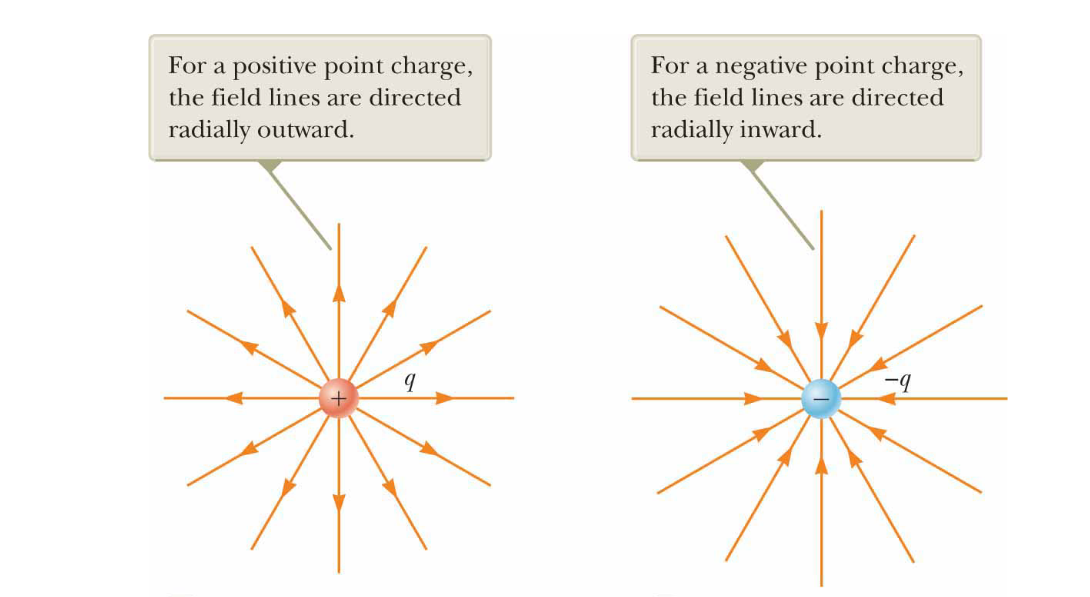
\includegraphics[scale=0.35]{electric_field_lines.png}
\end{center}


The density of the lines leaving or terminating at a particle is proportional to the charge of the particle.

\begin{equation*}
    \frac{N_2}{N_1} = |\frac{q_2}{q_1}|
\end{equation*}

Where $N$ is the number of field lines coming from a charge, and $q$ is the charge of that particle.\\

\begin{figure}[h]
    \centering
    \begin{subfigure}{0.4\textwidth}
        \centering
        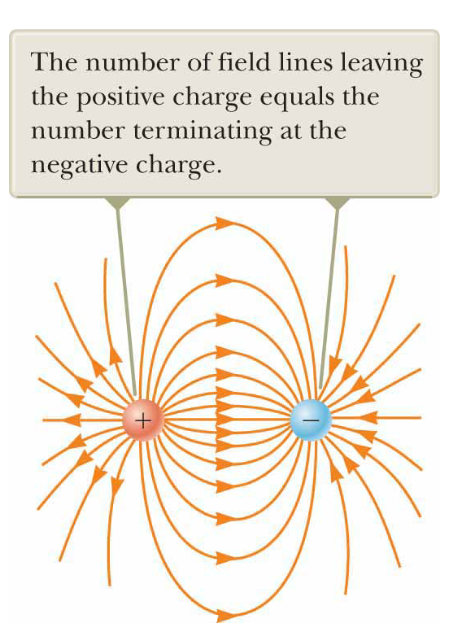
\includegraphics[scale=0.3]{electric_field_lines1.png}
        \caption{Field lines between two equal and opposite charges}
    \end{subfigure}%
    \hspace{0.1\textwidth}
    \begin{subfigure}{0.4\textwidth}
        \centering
        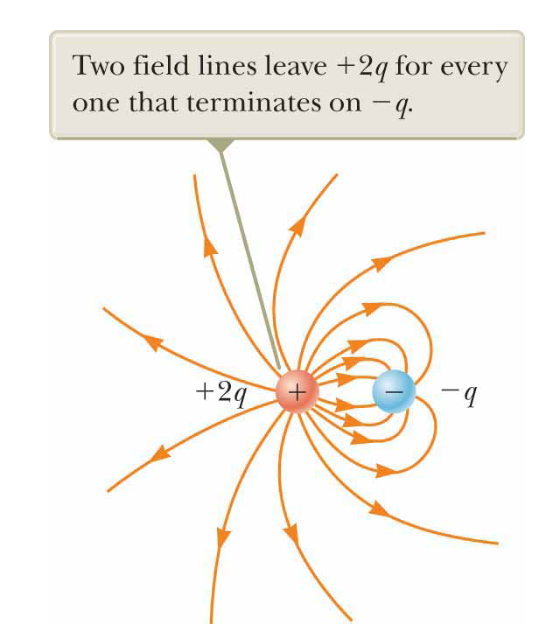
\includegraphics[scale=0.3]{electric_field_lines2.png}
        \caption{Field lines between two unequal and opposite charges}
    \end{subfigure}
\end{figure}

\hrulefill

\subsubsection*{Charge Density}
\paragraph*{Definition}
Charge density is the amount of charge per unit length ($\lambda$), area ($\sigma$), or volume ($\rho$) depending on the geometry of the object.

\begin{align*}
    \text{Linear Charge Density} : \lambda &= \frac{Q}{\ell} \Longrightarrow dq = \lambda d\ell\\
    \text{Surface Charge Density} : \sigma &= \frac{Q}{A} \Longrightarrow dq = \sigma dA\\
    \text{Volume Charge Density} : \rho &= \frac{Q}{V} \Longrightarrow dq = \rho dV
\end{align*}